
\documentclass[hyperref={pdfpagelabels=false},ngerman]{beamer}

% stop font warning
\let\Tiny=\tiny
\providecommand\thispdfpagelabel[1]{}

\usepackage[english]{babel}
\usepackage{lmodern}
\usepackage[T1]{fontenc}
\usepackage[utf8]{inputenc}
\usepackage{graphicx,import}
\usepackage{feynmp}
\DeclareGraphicsRule{*}{mps}{*}{} 
\DeclareGraphicsExtensions{.pdf}
\usepackage{amsmath,amssymb,amstext,amsfonts} % mathrsfs
\usepackage{array,booktabs,tabularx}
\usepackage{tikz,tikz-uml,pgf-pie}
\usetikzlibrary{shapes,calc,arrows,positioning}
\tikzstyle{block} = [rectangle, draw, text width=7em, text centered, minimum height=2em]
\tikzstyle{arrow} = [draw, -latex, thick]
\tikzstyle{arrow2} = [draw, latex-latex, thick]
\tikzstyle{quark}  = [rectangle, draw, fill=yellow, minimum width=2em, text centered, minimum height=2em]
\tikzstyle{lepton} = [rectangle, draw, fill=red!50, minimum width=2em, text centered, minimum height=2em]
\tikzstyle{gauge}  = [circle   , draw, fill=green , minimum size=2em, inner sep=0pt, text centered]
\tikzstyle{scalar} = [diamond  , draw, fill=blue!40, minimum width=2.3em, text centered, minimum height=2.3em, inner sep=0pt]
\tikzstyle{goldstone} = [diamond, draw, dashed, fill=blue!30, minimum width=2.3em, text centered, minimum height=2.3em, inner sep=0pt]
\tikzstyle{squark}   = [diamond, draw, fill=yellow, minimum width=2.3em, text centered, minimum height=2.3em, inner sep=0pt]
\tikzstyle{slepton}  = [diamond, draw, fill=red!50, minimum width=2.3em, text centered, minimum height=2.3em, inner sep=0pt]
\tikzstyle{gaugino}  = [rectangle, draw, fill=green , minimum size=2em, inner sep=0pt, text centered]
\tikzstyle{higgsino} = [rectangle, draw, fill=blue!40  , minimum width=2em, text centered, minimum height=2em]
\tikzstyle{inert}    = [diamond  , draw, fill=teal!80, minimum width=2.3em, text centered, minimum height=2.3em, inner sep=0pt]
\tikzstyle{inertino} = [rectangle, draw, fill=teal!80, minimum width=2em, text centered, minimum height=2em]
\tikzstyle{phantom}  = [rectangle, minimum width=2em, text centered, minimum height=2em]
\usepackage{slashed}
\usepackage{fixltx2e} % textsubscript
\usepackage{multirow}
\usepackage{tcolorbox}
\usepackage{pifont}
\usepackage{xspace}
\usepackage{hyperref}
\hypersetup{colorlinks,linkcolor=,urlcolor=blue}
\usepackage{listings}
\lstset{breaklines=true,
  breakatwhitespace=true,
%  numbers=left,
  numberstyle=\tiny,
  stepnumber=1,
  basicstyle=\ttfamily\footnotesize,
  commentstyle=\ttfamily\color{gray},
  postbreak={\mbox{{$\hookrightarrow$}}\space\space},
  breakindent=10pt,
  breakautoindent=false,
  showspaces=false,
  showstringspaces=false,
  frame=single}

\definecolor{darkgreen}{RGB}{0,176,0}

\newcommand{\cmark}{\ding{51}}%
\newcommand{\xmark}{\ding{55}}%
\newcommand{\fmfvcenter}[1]{\;\vcenter{\hbox{\fmfreuse{#1}}}\;}
\newcommand{\eh}[1]{\,\mathsf{#1}}
\newcommand{\ok}{\textcolor{darkgreen}{\cmark}}
\newcommand{\notok}{\textcolor{red}{\xmark}}
\newcommand{\maybe}{\textcolor{gray}{\cmark}}
\newcommand{\meh}{\textcolor{gray}{\textbf{\huge\lower.1em\hbox{-}}}}
\newcommand{\Lagr}{\mathcal{L}}
\newcommand{\MS}{\ensuremath{M_S}}
\newcommand{\mathi}{\mathsf{i}}
\newcommand{\mycite}[1]{\textcolor{darkgray}{\tiny [#1]}}
\newcommand{\bigcite}[1]{\textcolor{darkgray}{[#1]}}
\newcommand{\dimrep}[1]{\mathbf{#1}}
\newcommand{\dimrepadj}[1]{\mathbf{\overline{#1}}}
\newcommand{\ESSM}{E\textsubscript{6}SSM}
\newcommand{\CESSM}{CE\textsubscript{6}SSM}
\DeclareMathOperator{\tildeRe}{\widetilde Re}
\DeclareMathOperator{\sign}{sign}
\DeclareMathOperator{\re}{Re}
\DeclareMathOperator{\im}{Im}
\renewcommand{\emph}{\textbf}
\newcommand{\dd}{\mathsf{d}}
\newcommand{\myurl}[1]{\href{#1}{#1}}
\newcommand{\Superpot}{\mathcal{W}}
\newcommand{\SuperField}[1]{#1}
\newcommand{\ConjSuperField}[1]{\bar{#1}}
\newcommand{\UY}{\ensuremath{U(1)_{Y}}}
\newcommand{\UN}{\ensuremath{U(1)_{N}}}
\newcommand{\Uem}{\ensuremath{U(1)_\text{em}}}
\newcommand{\SUL}{\ensuremath{SU(2)_\text{L}}}
\newcommand{\SUc}{\ensuremath{SU(3)_\text{c}}}
\newcommand{\SOten}{\ensuremath{{SO(10)}}}
\newcommand{\comma}{,}
\newcommand{\DRbar}{\ensuremath{\overline{\text{DR}}}}
\newcommand{\MSbar}{\ensuremath{\overline{\text{MS}}}}
\newcommand{\SM}{\ensuremath{\text{SM}}}
\newcommand{\MSSM}{\ensuremath{\text{MSSM}}}
\newcommand{\pole}{\ensuremath{\text{pole}}}
\newcommand{\tree}{\ensuremath{\text{tree}}}
\newcommand{\fsstar}{\textbf{*}}
\newcommand{\Zv}{\ensuremath{\backslash\mkern-11.0mu{Z_3}}}
\newcommand{\downrightknickarrow}{\mathrel{\scalebox{1.3}{\rotatebox[origin=c]{180}{$\Lsh$}}}}
\newcommand{\threelinebrace}{$\left. \begin{array}{c} \\ \\ \\ \end{array} \right\rbrace$}
\newcommand{\fivelinebrace}{$\left. \begin{array}{c} \\ \\ \\ \\ \\ \end{array} \right\rbrace$}
\newcommand{\twolinebrace}{$\left. \begin{array}{c} \\ \\ \end{array} \right\rbrace$}
\newcommand{\elevenlinebrace}{$\left. \begin{array}{c} \\ \\ \\ \\ \\ \\ \\ \\ \\ \\ \\ \end{array} \right\rbrace$}
\newcommand{\at}{\alpha_t}
\newcommand{\ab}{\alpha_b}
\newcommand{\atau}{\alpha_\tau}
\newcommand{\as}{\alpha_s}

% set look of slides
\usetheme{Madrid}
\useoutertheme{default}
\useinnertheme{circles}
\usecolortheme{default}
\beamertemplatenavigationsymbolsempty % keine Navigationselemente
\setbeamersize{text margin left = 1cm, text margin right = 1cm}

% define footer
\makeatletter
\setbeamertemplate{footline}
{
  \hfill\hbox{\insertframenumber{} / \inserttotalframenumber\hspace*{4pt}}%
  \vskip3pt%
}
\makeatother
\usecolortheme{tud}

\title{Higgs mass prediction in supersymmetry with effective field theory techniques}

\author[Alexander Voigt]{Alexander Voigt}

\date{Heidelberg, 13.06.2017}

\institute[Aachen]{RWTH Aachen}
\subject{FlexibleSUSY,MSSM,Higgs,FlexibleEFTHiggs}
\keywords{FlexibleSUSY,MSSM,Higgs,FlexibleEFTHiggs}

%%%%%%%%%%%%%%%%%%%%%%%%%%%%%%%%%%%%%%%%%%%%%%%%%%%%%%%%%%%%%%%%%%%%%%%%%%%%%

\begin{document}

%%%%%%%%%%%%%%%%%%%%%%%%%%%%%%%%%%%%%%%%
\begin{frame}[plain]
  \tikz [remember picture,overlay]
  \node at
    ([yshift=1.3cm,xshift=4cm]current page.south)
    {\includegraphics[height=2cm]{images/RWTH_Logo}};
  \titlepage  
\end{frame}

%%%%%%%%%%%%%%%%%%%%%%%%%%%%%%%%%%%%%%%%
\begin{frame}{Contents}
  \tableofcontents
\end{frame}

\section{Introduction to supersymmetry}

\begin{frame}{Contents}
  \tableofcontents[currentsection]  
\end{frame}

\begin{frame}{Supersymmetry}
  Still an attractive extension of the Standard Model!\\[1em]
  \emph{Features:}
  \begin{itemize}
  \item can solve the hierarchy problem (heavy BSM particles can give
    large corrections to the Higgs mass)
  \item gauge coupling unification at $\sim 10^{16}\eh{GeV}$ (due to
    extra matter)
  \item possible connection to super-gravity models and string theory
    (\ESSM, MRSSM)
  \item can explain deviation of $(g-2)_\mu$
  \item can stabilize the electroweak vacuum (see later)
  \end{itemize}
  \vspace{1em}
  \emph{Problem:} LHC has not found any SUSY particles so far
  $\Rightarrow$ SUSY particles are probably heavy
\end{frame}

\begin{frame}{Minimal supersymmetry (MSSM)}
  MSSM = supersymmetric extension of the 2HDM \\[1em]
  Particle content (superfields):
  \begin{equation*}
    \begin{aligned}
      \hat{Q}  &:\textstyle (\mathbf{     3} ,\mathbf{2}, \frac{1}{6}) ,
      &\hat{u}^c&:\textstyle (\bar{\mathbf{3}},\mathbf{1},-\frac{2}{3}) ,
      &\hat{d}^c&:\textstyle (\bar{\mathbf{3}},\mathbf{1}, \frac{1}{3}) ,
      \\
      \hat{L}  &:\textstyle (\mathbf{     1} ,\mathbf{2},-\frac{1}{2}) ,
      &\hat{e}^c&:\textstyle (\mathbf{     1} ,\mathbf{1}, 1          ) ,
      \\
      \hat{H}_d&:\textstyle (\mathbf{     1} ,\mathbf{2},-\frac{1}{2}) ,
      &\hat{H}_u&:\textstyle (\mathbf{     1} ,\mathbf{2}, \frac{1}{2}) ,
      \\
      \tilde{B}  &:\textstyle (\mathbf{1},\mathbf{1},0) ,
      &\tilde{W}  &:\textstyle (\mathbf{1},\mathbf{3},0) ,
      &\tilde{g}  &:\textstyle (\mathbf{8},\mathbf{1},0)
    \end{aligned}
  \end{equation*}
  Superpotential:
  \begin{align*}
    \mathcal{W}_\MSSM &= (Y_u)_{ij} \, \hat{Q}_i\cdot\hat{H}_u \, \hat{u}^c_j
    + (Y_d)_{ij} \, \hat{Q}_i\cdot\hat{H}_{d} \, \hat{d}^c_j
    +  (Y_e)_{ij} \, \hat{L}_i\cdot\hat{H}_{d} \, \hat{e}^c_j \\
    &\phantom{={}} + \mu \hat{H}_u\cdot\hat{H}_{d}
  \end{align*}
\end{frame}

\begin{frame}{Minimal supersymmetry (MSSM)}
  SUSY particles have not been observed $\Rightarrow$ SUSY must be
  broken.  Here we consider soft breaking:
  \begin{align*}
    \mathcal{L}_{\MSSM}^\mathsf{soft} &= -\frac12\Big[M_1\bar{\tilde{B}}^0\tilde{B}^0 +
    M_2\bar{\tilde{W}}\tilde{W} +
    M_3\bar{\tilde{g}}\tilde{g}\Big] \\
    &\phantom{={}} - m^2_{H_u}|H_u|^2 - m^2_{H_d}|H_d|^2 - \Big[B\mu \, {H}_u\cdot{H}_{d} +
    \text{h.c.}\Big] \\
    &\phantom{={}}
    -\Big[\tilde{Q}_i^\dagger(m^2_Q)_{ij}\tilde{Q}_j +
    \tilde{d}_{Ri}^\dagger(m^2_d)_{ij}\tilde{d}_{Rj}
    +
    \tilde{u}_{Ri}^\dagger(m^2_u)_{ij}\tilde{u}_{Rj} \\
    &\phantom{={}}\qquad
    + \tilde{L}_{i}^\dagger(m^2_L)_{ij}\tilde{L}_{j} +
    \tilde{e}_{Ri}^\dagger(m^2_e)_{ij}\tilde{e}_{Rj}
    \Big] \\
    &\phantom{={}}
    +\Big[(T_u)_{ij}\tilde{Q}_i \cdot  H_u\tilde{u}^\dagger_{\text{R}j}
    +
    (T_d)_{ij}\tilde{Q}_i \cdot H_{d} \tilde{d}^\dagger_{\text{R}j}
    + (T_e)_{ij}\tilde{L}_i \cdot H_{d}\tilde{e}^\dagger_{\text{R}j} \\
    &\phantom{={}} \qquad + \text{h.c.}\Big]
  \end{align*}
\end{frame}

\begin{frame}{Higgs sector of the MSSM}
  The two Higgs doublets develop VEVs as
  \begin{align*}
    H_d &=
    \begin{pmatrix}
      \frac{v_d}{\sqrt{2}} + H_d^0 \\ H_d^-
    \end{pmatrix} &
    H_u &=
    \begin{pmatrix}
      H_u^+ \\ \frac{v_u}{\sqrt{2}} + H_u^0
    \end{pmatrix}
  \end{align*}
  $\Rightarrow$
  \begin{align*}
    m_Z^2 &= \frac{1}{2} (g_Y^2 + g_2^2) v^2, &
    m_W^2 &= \frac{1}{2} g_2^2 v^2, \\
    m_t &= y_t v_u / \sqrt{2}, &
    m_t &= y_b v_d / \sqrt{2}, \\
    v^2 &:= v_u^2 + v_d^2, & \tan\beta &:= v_u/v_d
  \end{align*}
  Mixing of Higgs fields:
  \begin{align*}
    \left(\re H_d^0, \re H_u^0\right) &\rightarrow (h, H) \\
    \left(\im H_d^0, \im H_u^0\right) &\rightarrow (G^0, A) \\
    \left((H_d^-)^*, H_u^+\right)     &\rightarrow (G^+, H^+)
  \end{align*}
\end{frame}

\begin{frame}{Considered SUSY scenarios}
  In the following I set for simplicity
  \begin{align*}
    \begin{split}
      &(m_f^2)_{ij}(\MS) = \delta_{ij} \MS^2, \quad (f=Q,u,d,L,e) \\
      &M_i(\MS) = \MS, \quad (i = 1,2,3) \\
      &\mu(\MS) = \MS , \\
      &m_A^2(\MS) = \frac{B\mu(\MS)}{\sin\beta(\MS) \cos\beta(\MS)} = \MS^2 , \\
      &(X_f)_{ij}(\MS) = (T_f)_{ij}/(Y_f)_{ij} - 
      \begin{Bmatrix}
        \mu^*\tan\beta \\ \mu^*\cot\beta
      \end{Bmatrix}
      \quad \text{for} \quad \left\{
        \begin{array}{l}\!\!f = d, e, \\ \!\!f = u,
        \end{array}
      \right.
    \end{split}
  \end{align*}
  Abbreviations:\\[0.5em]
  $X_t := (X_u)_{33}$, $X_b := (X_d)_{33}$, $X_\tau := (X_e)_{33}$,\\
  $s_\beta := \sin\beta$, $c_\beta := \cos\beta$
\end{frame}

\begin{frame}{Current limits on SUSY particle masses}
  \begin{center}
    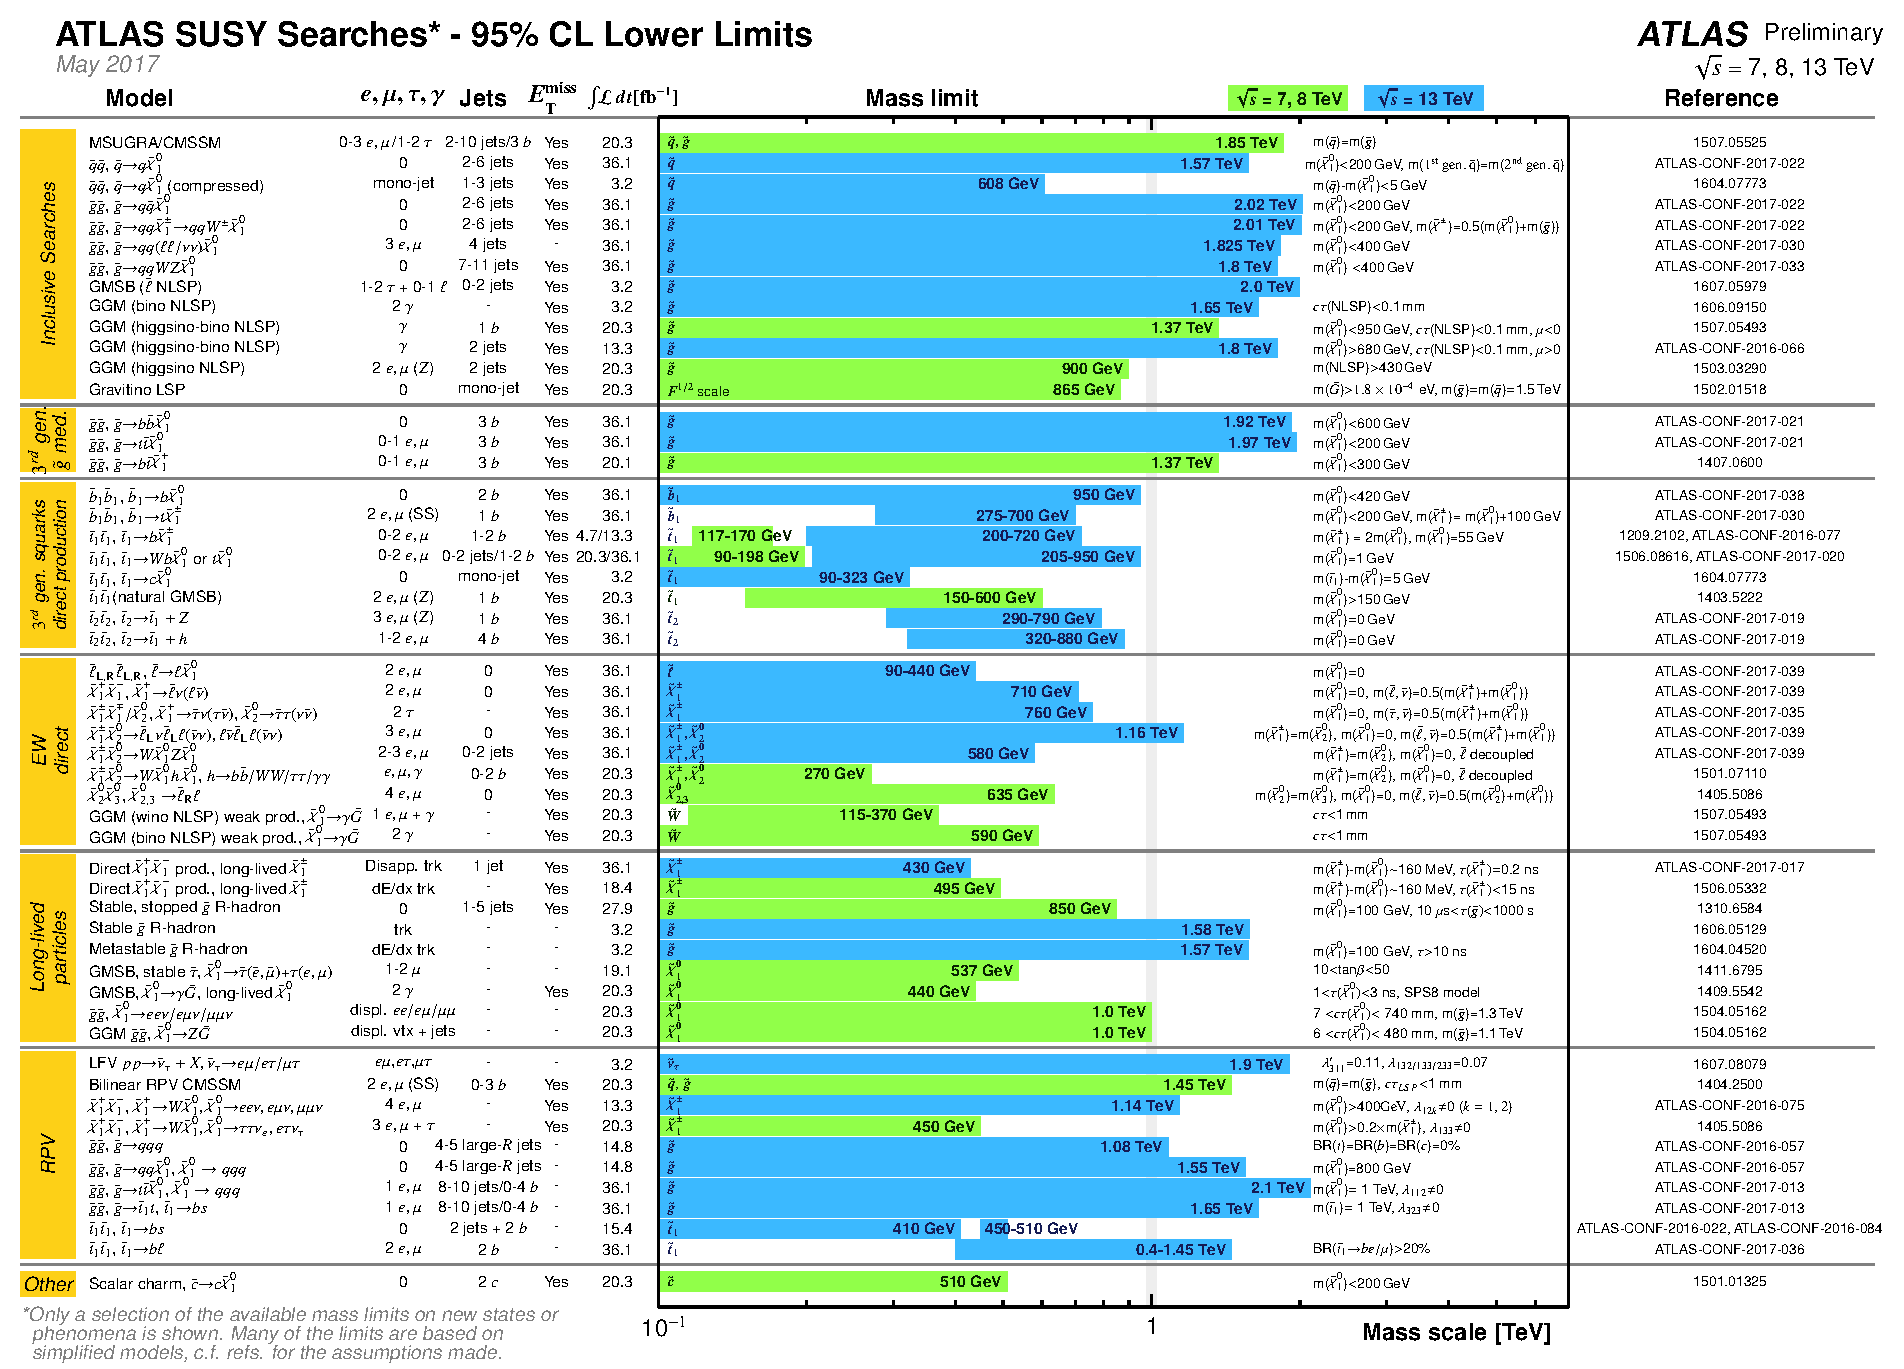
\includegraphics[width=\textwidth]{images/ATLAS_SUSY_Summary}
  \end{center}
\end{frame}

%%%%%%%%%%%%%%%%%%%%%%%%%%%%%%%%%%%%%%%%

\section{Higgs mass calculation in the MSSM}

\subsection{Higgs mass calculation at fixed loop order}

\begin{frame}{Contents}
  \tableofcontents[
  currentsection,
  currentsubsection,
  subsectionstyle=show/shaded/hide]  
\end{frame}

\begin{frame}{Higgs mass in the CP-conserving MSSM}
  \begin{align*}
    M =
    \begin{pmatrix}
      m_A^2 s_\beta^2 + m_Z^2 c_\beta^2 & -(m_A^2 + m_Z^2) s_\beta c_\beta \\
      \cdot & m_A^2 c_\beta^2 + m_Z^2 s_\beta^2
    \end{pmatrix}
  \end{align*}
  $\Rightarrow$
  \begin{align*}
    m_{h,H}^2 = \frac{1}{2} \left[
      m_Z^2 + m_A^2 \mp \sqrt{(m_Z^2 + m_A^2)^2 - 4 m_Z^2 m_A^2 c_{2\beta}^2}
    \right]
  \end{align*}
  $\Rightarrow$
  \begin{align*}
    m_h^2 < \min(m_Z^2, m_A^2) c_{2\beta}^2
  \end{align*}
  If $m_A \gg m_Z$:
  \begin{align*}
    m_h^2 \approx \frac{1}{4} (g_Y^2 + g_2^2) (v_u^2 + v_d^2) c_{2\beta}^2
    = m_Z^2 c_{2\beta}^2
  \end{align*}
\end{frame}

\begin{frame}{Higgs mass in the CP-conserving MSSM}
  \begin{align*}
    m_h^2 \approx \frac{1}{4} (g_Y^2 + g_2^2) (v_u^2 + v_d^2) c_{2\beta}^2
    = m_Z^2 c_{2\beta}^2
  \end{align*}
  In the MSSM the tree-level Higgs mass is restricted to be smaller
  than $m_Z$!
  \\[2em]
  Q: How can $M_h \approx 125\eh{GeV}$ be possible in the MSSM? \\[1em]
  A: Large loop corrections are to be expected!
  \begin{align*}
    M_h^2 &= m_h^2 + \Delta m_h^2
    & &\Rightarrow &
    \Delta m_h^2 &\geq (85\eh{GeV})^2
  \end{align*}
\end{frame}

% Savebox which contains the the Feynman rules
\newsavebox{\feynmanrules}
\sbox{\feynmanrules}{
\begin{fmffile}{Feynman/higgs} % file name and path
  \fmfset{thin}{.8pt}
  \fmfset{wiggly_len}{5mm}
  \fmfset{dash_len}{2.5mm}
  \fmfset{dot_size}{1thick}
  \fmfset{arrow_len}{2.5mm}
  \fmfset{curly_len}{2.5mm}

\begin{fmfgraph*}(60,60)
  \fmfkeep{htop}
  \fmfleft{v1}
  \fmfright{v2}
  \fmf{higgs}{v1,c1}
  \fmf{higgs}{c2,v2}
  \fmf{quark,left,tension=0.5,label=$t$}{c1,c2}
  \fmf{quark,left,tension=0.5}{c2,c1}
\end{fmfgraph*}

\begin{fmfgraph*}(60,60)
  \fmfkeep{hstop}
  \fmfleft{v1}
  \fmfright{v2}
  \fmf{higgs}{v1,c1}
  \fmf{higgs}{c2,v2}
  \fmf{scalar,left,tension=0.5,label=$\tilde{t}_i$}{c1,c2}
  \fmf{scalar,left,tension=0.5}{c2,c1}
\end{fmfgraph*}

\begin{fmfgraph*}(60,60)
  \fmfkeep{hstopA}
  \fmfleft{v1}
  \fmfright{v2}
  \fmf{higgs}{v1,c,v2}
  \fmf{scalar,right,tension=0.8,label=$\tilde{t}_i$}{c,c}
\end{fmfgraph*}

\begin{fmfgraph*}(60,60)
  \fmfkeep{htoptad}
  \fmfleft{v1}
  \fmfright{v2}
  \fmftop{t1}
  \fmf{higgs}{v1,c,v2}
  \fmffreeze
  \fmf{higgs}{c,c1}
  \fmf{quark,right,tension=0.3,label=$t$}{c1,c2}
  \fmf{quark,right,tension=0.3}{c2,c1}
  \fmf{phantom,tension=10}{c2,t1}
\end{fmfgraph*}

\begin{fmfgraph*}(60,60)
  \fmfkeep{hstoptad}
  \fmfleft{v1}
  \fmfright{v2}
  \fmftop{t1}
  \fmf{higgs}{v1,c,v2}
  \fmffreeze
  \fmf{higgs}{c,c1}
  \fmf{scalar,right,tension=0.3,label=$\tilde{t}_i$}{c1,c2}
  \fmf{scalar,right,tension=0.3}{c2,c1}
  \fmf{phantom,tension=10}{c2,t1}
\end{fmfgraph*}
\end{fmffile}
}

\begin{frame}{Higgs mass at 1-loop level}
  In the MSSM the following diagrams give the dominant contribution to
  $M_h$ at the 1-loop level:
  \begin{align*}
    (\Delta m_h^2)^{1L} &= -\Sigma_h^{1L}(p^2) + \frac{t_h^{1L}}{v} \\
    &= \fmfvcenter{htop} + \fmfvcenter{hstop} + \fmfvcenter{hstopA} \\
    &\phantom{={}} + \fmfvcenter{htoptad} + \fmfvcenter{hstoptad} \\
    &\approx \frac{12 m_t^2 y_t^2}{(4\pi)^2} \left(
      \ln\frac{m_{\tilde{t}}^2}{m_t^2}
      + \frac{X_t^2}{m_{\tilde{t}}^2}
      - \frac{X_t^4}{12 m_{\tilde{t}}^4}
    \right)
    \quad \text{for} \quad m_{\tilde{t}_1} = m_{\tilde{t}_2}, p^2 = 0
  \end{align*}
\end{frame}

\begin{frame}{Higgs mass at 1-loop level}
  \begin{align*}
    (\Delta m_h^2)^{1L} &\approx
    \frac{12 m_t^2 y_t^2}{(4\pi)^2} \left(
      \ln\frac{m_{\tilde{t}}^2}{m_t^2}
      + \frac{X_t^2}{m_{\tilde{t}}^2}
      - \frac{X_t^4}{12 m_{\tilde{t}}^4}
    \right) + O(p^2)
  \end{align*}
  $X_t = A_t - \mu/t_\beta$ = stop mixing parameter
  % 24 mt^4 / (16 Pi^2 v^2) (Log[MS^2/mt^2] + Xt^2/MS^2 - Xt^4/(12 MS^4))
  \\[1em]
  \emph{Observations:}
  \begin{itemize}
  \item logarithmically enhanced by $m_{\tilde{t}} / m_t$
  \item maximal for $X_t \approx \sqrt{6} m_{\tilde{t}}$
  \item high sensitivity on $m_t$, due to effective prefactor $m_t^4$
  \item ambiguity of definition of $m_t$: pole mass or \DRbar\ mass? \\
    $M_t \approx 173.3\eh{GeV}$, $m_t^{\DRbar} \approx 165\eh{GeV}$ \\
    $\Rightarrow$ huge theoretical uncertainty!\\
    $\Rightarrow$ 2-loop calculation needed to resolve this ambiguity
  \item to get $M_h \approx 125\eh{GeV}$, $m_{\tilde{t}} \gtrsim 1\eh{TeV}$ needed
    (see later)
  \end{itemize}
\end{frame}

\begin{frame}{Higgs mass at 2-loop level}
  Known contributions: $O(\as (\at + \ab) + (\at+\ab)^2 + \atau^2)$ for $p^2 = 0$
  \\[1em]
  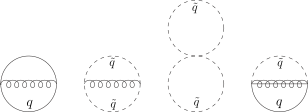
\includegraphics[width=0.6\textwidth]{images/atas}\\[1em]
  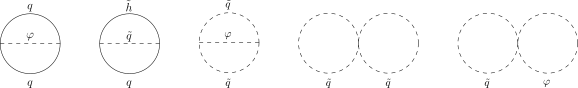
\includegraphics[width=\textwidth]{images/atat}
\end{frame}

\begin{frame}{Higgs mass at 2-loop level}
  \begin{align*}
    (\Delta m_h^2)^{2L} &\approx
    \frac{m_t^2 y_t^4}{(4\pi)^4} \left(
      c_1 \ln^2\frac{\MS^2}{m_t^2}
      + c_2 \ln\frac{\MS^2}{m_t^2}
      + c_3
    \right) \\
    & +
    \frac{m_t^2 y_t^2 g_3^2}{(4\pi)^4} \left(
      c_4 \ln^2\frac{\MS^2}{m_t^2}
      c_5 \ln\frac{\MS^2}{m_t^2}
      + c_6
    \right)
  \end{align*}
  \emph{Facts:}
  \begin{itemize}
  \item logarithmically enhanced by $\MS / m_t$
  \item still high sensitivity on $m_t$
  \item ambiguity of definition of $m_t$ is resolved
  \item ambiguity of definition of $\as$: $\as^\SM(M_Z)$, $\as^\MSSM(\MS)$, \ldots ? \\
    $\Rightarrow$ 3-loop calculation needed to resolve this ambiguity
  \end{itemize}
\end{frame}

\begin{frame}{Higgs mass at 3-loop level}
  Known contributions: $O(\at\as^2)$ for $p^2 = 0$ \mycite{arXiv:1005.5709}
  \begin{align*}
    (\Delta m_h^2)^{3L} &\approx
    \frac{m_t^2 y_t^2 g_3^4}{(4\pi)^6} \left(
      c_7 \ln^3\frac{\MS^2}{m_t^2}
      + c_8 \ln^2\frac{\MS^2}{m_t^2}
      + c_9 \ln\frac{\MS^2}{m_t^2}
      + c_{10}
    \right)
  \end{align*}
  \emph{Facts:}
  \begin{itemize}
  \item logarithmically enhanced by $\MS / m_t$
  \item still high sensitivity on $m_t$
  \item ambiguity of definition of $m_t$ is resolved
  \item ambiguity of definition of $\as$ is resolved
  \end{itemize}
\end{frame}

\begin{frame}{Summary of loop calculations}
  Typical order of magnitude of loop contributions (depends on
  parameter scenario):
  \begin{align*}
    M_h &= m_h + \Delta m_h^{1L} + \Delta m_h^{2L} + \Delta m_h^{3L} + \cdots \\
    &\approx [91 + O(20\ldots 30) + O(2\ldots 4) + O(1\ldots 2)] \eh{GeV}
  \end{align*}
  \emph{Advantages:}
  \begin{itemize}
  \item includes logarithmic, non-logarithmic and suppressed terms of
    the order $O(v^2/\MS^2)$ at fixed loop order
  \item Precise prediction if $\MS \sim m_t$
  \end{itemize}
  \emph{Problem:}
  \begin{itemize}
  \item large corrections, if $\MS \gg m_t$ \\
    $\Rightarrow$ slow convergence of perturbation series \\
    $\Rightarrow$ large theoretical uncertainty, ($1$--$2\eh{GeV}$, or
    more) \\
    $M_h^{\text{exp}} = (125.09 \pm 0.24)\eh{GeV}$
  \end{itemize}
\end{frame}

%%%%%%%%%%%%%%%%%%%%%%%%%%%%%%%%%%%%%%%%

\subsection{Higgs mass calculation in an EFT}

\begin{frame}{Contents}
  \tableofcontents[
  currentsection,
  currentsubsection,
  subsectionstyle=show/shaded/hide]  
\end{frame}

\begin{frame}{Higgs mass calculation in an EFT}
  \emph{Idea:} Integrate out SUSY particles at $\MS$ (expand in $v^2/MS^2$) \\
  $\Rightarrow$ $\lambda(\MS)$ is fixed by the MSSM \\
  $\Rightarrow$ effectively separation of scales $\MS$ and $M_t$.
  \begin{center}
    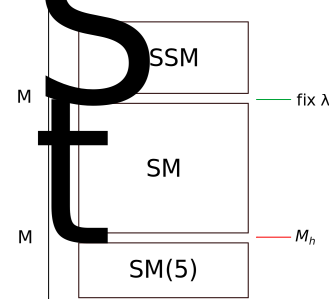
\includegraphics[width=0.5\textwidth]{images/mssm-sm-tower-eft}
  \end{center}
\end{frame}

\begin{frame}{EFT procedure}
  Match all renormalized $n$-point functions at $p^2 = v^2 = 0$, $Q =
  \MS$ of the SM and MSSM:
  \begin{align*}
    \partial_{p^2}^{(k)}\Gamma_{h,\ldots,h}^{\MSSM,(n)}
    = \partial_{p^2}^{(k)}\Gamma_{h,\ldots,h}^{\SM,(n)}
  \end{align*}
  $\Rightarrow$
  \begin{align*}
    \lambda(M_S) &= \frac{1}{4}\left[g_Y^{2} + g_2^2\right] \cos^22\beta
    + \Delta \lambda
  \end{align*}
  RG running of $\lambda(\MS)$ to $Q=M_t$.\\
  Calculation of $M_h$ in the Standard Model:
  \begin{align*}
    (M_h^\SM)^2 &= \lambda(M_t) v^2 + (\Delta m_h^2)^{1L}
    + (\Delta m_h^2)^{2L} + \cdots
  \end{align*}
\end{frame}

\begin{frame}{Concrete EFT example}
  \begin{enumerate}
  \item Calculate $\lambda$ at $Q = \MS$:
    \begin{align*}
      \lambda(Q) &= \frac{1}{4}\left[g_Y^{2} + g_2^2\right] c^2_{2\beta}
      + \frac{12 m_t^2 y_t^2}{(4\pi)^2 v^2} \left[
        \ln\frac{\MS^2}{Q^2} + \frac{X_t^2}{\MS^2} - \frac{X_t^4}{12 \MS^4}
      \right]
      + \cdots
    \end{align*}
    $\Rightarrow$ \textcolor{darkgreen}{no large logs}
  \item RG running from $Q = \MS$ $\rightarrow M_t$.\\
    $\Rightarrow$ \textcolor{darkgreen}{logs are resummed to all orders}
  \item Calculate $M_h$ in the SM at $Q = M_t$:
    \begin{align*}
      (M_h^\SM)^2 &= \lambda v^2 + \frac{12 m_t^2 y_t^2}{(4\pi)^2 v^2} \ln\frac{Q^2}{m_t^2} + \cdots
    \end{align*}
    $\Rightarrow$ \textcolor{darkgreen}{no large logs}
  \end{enumerate}
\end{frame}

\begin{frame}{Summary of EFT approach}
  Typical order of magnitude of loop contributions (depends on
  parameter scenario, here $X_t = 0$, $\MS = 20\eh{TeV}$):
  \begin{align*}
    M_h &= m_h + \Delta m_h^{1L} + \Delta m_h^{2L} + \cdots \\
    &= \sqrt{\lambda(M_t)} v + \Delta m_h^{1L} + \Delta m_h^{2L} + \cdots \\
    &\approx [O(124) + O(0.5\ldots 1) + O(0.1\ldots 0.2)] \eh{GeV}\\
    &= \sqrt{\lambda(\MS)} v + \text{logs} + \Delta m_h^{1L} + \Delta m_h^{2L} + \cdots \\
    &\approx [O(84) + O(40) + O(0.5\ldots 1) + O(0.1\ldots 0.2)] \eh{GeV}
  \end{align*}
  \emph{Advantages:}
  \begin{itemize}
  \item large logarithmic loop corrections are avoided
  \item large logarithms $\propto\ln(M_S/M_t)$ are resummed to all orders
  \end{itemize}
  \emph{Disadvantage:} usually terms $O(v^2/M_S^2)$ are neglected \\
  $\Rightarrow$ imprecise when $v \sim \MS$
  $\Rightarrow$ large theoretical uncertainty
\end{frame}

\begin{frame}{Summary}
  \begin{center}
    \begin{tabular}{lcc}
      \toprule
                  & low $\MS$ & high $\MS$ \\
                  & $\MS \lesssim 2\eh{TeV}$ & $\MS \gtrsim 2\eh{TeV}$ \\
      \midrule
      fixed-order & \ok       & \notok     \\
      EFT         & \notok    & \ok        \\
      ? mixed     & \ok       & \ok        \\
      \bottomrule
    \end{tabular}
  \end{center}
  \vspace{2em}
  Q: Can the fixed-order and EFT approaches be combined? \\[1em]
  A: Yes!  \mycite{arXiv:1312.4937, arXiv:1609.00371}
\end{frame}

%%%%%%%%%%%%%%%%%%%%%%%%%%%%%%%%%%%%%%%%

\subsection{Higgs mass calculation in a mixed approach}

\begin{frame}{Contents}
  \tableofcontents[
  currentsection,
  currentsubsection,
  subsectionstyle=show/shaded/hide]  
\end{frame}

\begin{frame}{Mixed fixed-order and EFT approaches}
  \emph{Goal:} resum large logarithms and include suppressed
  $O(v^2/\MS^2)$ terms
  \\[2em]
  \emph{Two known approaches:}
  \begin{itemize}
  \item FeynHiggs \mycite{arXiv:1312.4937}: Replace logs from
    fixed-order calculation by resummed logs
    \begin{align*}
      M_h^2 = (M_h^2)_{\text{fixed-order}} - (M_h^2)_{\text{logs}} + (M_h^2)_{\text{resummed logs}}
    \end{align*}
  \item FlexibleEFTHiggs \mycite{arXiv:1609.00371}: Incorporate
    $O(v^2/\MS^2)$ terms into $\lambda$ by using the matching
    condition
    \begin{align*}
      (M_h^2)_{\SM} = (M_h^2)_{\MSSM} \qquad \text{at 1L level at } Q = \MS
    \end{align*}
  \end{itemize}
\end{frame}

\begin{frame}{FlexibleEFTHiggs approach}
  \emph{Idea:}
  \begin{enumerate}
  \item Determine $\lambda(\MS)$ from the condition
    \begin{align*}
      (M_h^2)_{\SM} &= (M_h^2)_{\MSSM}\qquad \text{1L, } Q = \MS
    \end{align*}
    \textcolor{darkgreen}{No suppressed terms are neglected.
      $\Rightarrow$ $\lambda$ contains all $O(v^2/\MS^2)$ suppressed
      terms}
  \item RG running of $\lambda(\MS)$ from $\MS \rightarrow M_t$\\
    \textcolor{darkgreen}{Note: $M_h$ is RG invariant.}
  \item Calculate $M_h$ in the Standard Model at $Q = M_t$:
    \begin{align*}
      M_h^2 = \lambda(M_t) v^2 + (\Delta m_h^2)^{1L}_{\SM}
    \end{align*}
    \textcolor{darkgreen}{$\Rightarrow$ $M_h$ contains all suppressed
      terms.}
  \end{enumerate}
\end{frame}

\begin{frame}{FlexibleEFTHiggs -- EFT equivalence}
  \begin{align*}
    (M_h^2)_{\SM} &= (M_h^2)_{\MSSM} \qquad \text{1L, } Q = \MS \\
    \lambda v^2 + (\Delta m_h^2)^{1L}_{\SM} &= (M_h^2)_{\MSSM}
  \end{align*}
  $\Rightarrow$
  \begin{align*}
    \lambda(\MS) &= \frac{1}{v^2} \left[ (M_h^2)_{\MSSM} - (\Delta m_h^2)^{1L}_{\SM} \right] \\
    &= \frac{1}{v^2} \left[
      (m_h^2)_{\MSSM} + (\Delta m_h^2)^{1L}_{\MSSM} - (\Delta m_h^2)^{1L}_{\SM}
    \right]
  \end{align*}
\end{frame}

\begin{frame}{FlexibleEFTHiggs -- EFT equivalence}
  Inserting 1-loop corrections to $(M_h^2)_{\MSSM}$ for $X_t = 0$:
  \begin{align*}
    \lambda(\MS) &=
    \frac{1}{v^2} \Bigg[
      \frac{1}{4}(g_Y^2 + g_2^2) v^2 c_{2\beta}^2 \\
      &\quad\qquad \textcolor{red}{ + \frac{c_{\alpha}^2}{s_{\beta}^2} (\Delta m_h^2)^{1L}_{\SM}
        - \frac{c_{\alpha}^2}{s_{\beta}^2} \frac{12 (y_t^{\SM})^2 m_t^2}{(4\pi)^2}
      B_0(p^2,\MS^2,\MS^2) } \\
      &\quad\qquad - (\Delta m_h^2)^{1L}_{\SM}
    \Bigg]
  \end{align*}
\end{frame}

\begin{frame}{FlexibleEFTHiggs -- EFT equivalence}
  In the decoupling limit $c_{\alpha}^2/s_{\beta}^2\rightarrow 1$:
  \begin{align*}
    \lambda(\MS) &=
    \frac{1}{4}(g_Y^2 + g_2^2) c_{2\beta}^2
    - 12 \frac{m_t^2 (y_t^{\SM})^2}{(4\pi)^2 v^2} B_0(p^2,\MS^2,\MS^2) \\
    &= \frac{1}{4} (g_Y^2 + g_2^2) c_{2\beta}^2
    - 12 \frac{m_t^2 (y_t^\SM)^2}{(4\pi)^2 v^2} \Bigg[ 
    -\log\frac{\MS^2}{Q^2} + \frac{p^2}{6\MS^2} + O\Big(\frac{p^4}{\MS^4}\Big)
    \Bigg] \\
    &= \frac{1}{4} (g_Y^2 + g_2^2) c_{2\beta}^2
    + 12 \frac{m_t^2 (y_t^\SM)^2}{(4\pi)^2 v^2} \Bigg[ 
    \log\frac{\MS^2}{Q^2} \Bigg] + O\Big(\frac{p^2}{\MS^2}\Big) \\
    &= \lambda^{\text{tree}}(\MS) + \lambda^{1L}(\MS) + O\Big(\frac{p^2}{\MS^2}\Big)
  \end{align*}
  $\lambda(\MS)$ in the FlexibleEFTHiggs approach is equivalent to the
  EFT approach at 1-loop, up to suppressed terms $O(v^2/\MS^2)$
\end{frame}

\begin{frame}{Summary FlexibleEFTHiggs approach}
  \begin{align*}
    (M_h^2)_{\SM} &= (M_h^2)_{\MSSM} \qquad \text{1L, } Q = \MS
\intertext{$\Rightarrow$}
    \lambda(\MS) &=
    \lambda^{\text{tree}}(\MS) + \lambda^{1L}(\MS) + O(v^2/\MS^2)
  \end{align*}
  \emph{Observations:}
  \begin{itemize}
  \item large 1-loop logarithms cancel in matching condition
  \item for $v=p=0$ FlexibleEFTHiggs is identical to a 1-loop EFT
    calculation
  \item all suppressed terms are incorporated in $\lambda$
  \item RG running resums (N)LL to all orders
  \end{itemize}
  \textcolor{darkgreen}{$\Rightarrow$ FlexibleEFTHiggs leads to a
    correct Higgs mass prediction at the full 1-loop level (including
    suppressed terms) with additional (N)LL resummation.}
\end{frame}

\begin{frame}{Comparison of approaches}
  \begin{center}
    \includegraphics[width=0.49\textwidth]{{{plots/uncertainties/Mh_MS_TB-5_Xt-0}}}
    \hfill
    \includegraphics[width=0.49\textwidth]{{{plots/FlexibleEFTHiggs-2/scan_Mh_Xt_TB-5_MS-2000}}}
  \end{center}
\end{frame}

%%%%%%%%%%%%%%%%%%%%%%%%%%%%%%%%%%%%%%%%

\section{Uncertainty estimate}

\begin{frame}{Contents}
  \tableofcontents[currentsection]  
\end{frame}

\begin{frame}{Ways to estimate the theoretical uncertainty}
  \emph{Good ansatz:} Change the calculation by higher orders beyond
  the calculational accuracy.
  \\
  \emph{Examples:}
  \begin{itemize}
  \item variation of the unphysical renormalization scale(s)
  \item change $m_t$ or $\as$ by higher orders
  \item re-parametrization of $M_h$
  \end{itemize}
  % \vspace{1em}
  \emph{Potential pitfalls:}
  \begin{itemize}
  \item some changes alone are an under-estimation of the uncertainty
    $\rightarrow$ a combination of multiple changes should be used
  \item potential over-estimation of the uncertainty when large
    cancellations occur at higher orders
  \item some changes are sensitive to the same kind of higher order
    contributions $\rightarrow$ potential double counting
  \item new higher order dependencies might be difficult to estimate\\
    Example: estimation of $\as$-dependence at 2-loop level when a
    2-loop calculation is not available
  \end{itemize}
\end{frame}

\begin{frame}{Example: under-estimation of the uncertainty}
  The variation of the renormalization alone might be an
  under-estimation of the uncertainty:
  \begin{center}
    \includegraphics[width=0.8\textwidth]{plots/SPheno-FS-uncertainty/scale_MSSM_yt_variants}
  \end{center}
\end{frame}

\begin{frame}{Example: over-estimation of the uncertainty}
  When large cancellations between the same kind of corrections from
  different sources occur, including only one source might lead to an
  over-estimation:
  \begin{center}
    \includegraphics[width=0.8\textwidth]{plots/contributions/scan_Mh_MS_TB-5_Xt-0_contributions}
  \end{center}
\end{frame}

\begin{frame}{Higgs mass uncertainty estimate}
  \emph{fixed-order:}
  \begin{itemize}
  \item $|M_h^{2L}(Q_\pole = \MS/2) - M_h^{2L}(Q_\pole = 2\MS)|$
  \item $|M_h^{2L}(y_t^{1L}) - M_h^{2L}(y_t^{2L})|$
  \end{itemize}
  \emph{EFT (SUSYHD):}
  \begin{itemize}
  \item $|M_h^{2L}(Q_\pole = M_t/2) - M_h^{2L}(Q_\pole = 2M_t)|$
  \item $|M_h^{2L}(y_t^{2L}) - M_h^{2L}(y_t^{3L})|$
  \item $|M_h^{2L}(Q_{\text{match}} = \MS/2) - M_h^{2L}(Q_{\text{match}} = 2\MS)|$
  \item $|M_h^{2L} - M_h^{2L}(\lambda \rightarrow \lambda(1 + v^2/\MS^2))|$
  \end{itemize}
  \emph{FlexibleEFTHiggs:}
  \begin{itemize}
  \item $|M_h^{2L}(Q_\pole = M_t/2) - M_h^{2L}(Q_\pole = 2M_t)|$
  \item $|M_h^{2L}(y_t^{2L}) - M_h^{2L}(y_t^{3L})|$
  \item $|M_h^{2L}(Q_{\text{match}} = \MS/2) - M_h^{2L}(Q_{\text{match}} = 2\MS)|$
  \end{itemize}
\end{frame}

\begin{frame}{Higgs mass uncertainty estimate}
  \begin{center}
    % \includegraphics[width=0.49\textwidth]{{{plots/uncertainties/Mh_MS_TB-5_Xt-0}}}
    \includegraphics[width=0.7\textwidth]{{{plots/uncertainties/DMh_MS_TB-5_Xt-1}}}
  \end{center}
\end{frame}

%%%%%%%%%%%%%%%%%%%%%%%%%%%%%%%%%%%%%%%%

\section{Summary}

\begin{frame}{Summary}
  \emph{Supersymmetry} is still viable, but LHC continuously excludes
  light SUSY scenarios\\[1em]
  %
  \emph{Approaches to calculate $M_h$}:
  \begin{center}
    \begin{tabular}{lcc}
      \toprule
                  & low $\MS$ & high $\MS$ \\
                  & $\MS \lesssim 2\eh{TeV}$ & $\MS \gtrsim 2\eh{TeV}$ \\
      \midrule
      fixed-order & \ok       & \notok     \\
      EFT         & \notok    & \ok        \\
      mixed       & \ok       & \ok        \\
      \bottomrule
    \end{tabular}
  \end{center}
  \emph{Uncertainty of $M_h$ in SUSY:}
  \begin{itemize}
  \item tricky to estimate and still ongoing effort!
  \item $\Delta M_h \gtrsim 1$--$2\eh{GeV}$ at least, but continuously
    improves
  \end{itemize}
\end{frame}

%%%%%%%%%%%%%%%%%%%%%%%%%%%%%%%%%%%%%%%%
% backup slides
%%%%%%%%%%%%%%%%%%%%%%%%%%%%%%%%%%%%%%%%

\begin{frame}[noframenumbering]
  \begin{center}
    \Huge Backup
  \end{center}
\end{frame}

%%%%%%%%%%%%%%%%%%%%%%%%%%%%%%%%%%%%%%%%

\begin{frame}[noframenumbering]{Numerical comparison}
  \begin{figure}
    \centering
    \includegraphics[width=\textwidth]{plots/FlexibleEFTHiggs/Mh_MS_TB-5_Xt-0}
  \end{figure}
  $\tan\beta = 5$, $X_{t,b,\tau} = 0$
\end{frame}

\begin{frame}[noframenumbering]{Numerical comparison}
  \begin{figure}
    \centering
    \includegraphics[width=\textwidth]{plots/FlexibleEFTHiggs/Mh_relative_MS_TB-5_Xt-0}
  \end{figure}
  $\tan\beta = 5$, $X_{t,b,\tau} = 0$
\end{frame}

\begin{frame}[noframenumbering]{Numerical comparison}
  \begin{figure}
    \centering
    \includegraphics[width=\textwidth]{plots/FlexibleEFTHiggs/Mh_Xt_TB-5_MS-2000}
  \end{figure}
  $\tan\beta = 5$, $M_S = 2 \eh{TeV}$, $X_{b,\tau} = 0$
\end{frame}

\begin{frame}[noframenumbering]{Numerical comparison}
  \begin{figure}
    \centering
    \includegraphics[width=\textwidth]{plots/FlexibleEFTHiggs/Mh_relative_Xt_TB-5_MS-2000}
  \end{figure}
  $\tan\beta = 5$, $M_S = 2 \eh{TeV}$, $X_{b,\tau} = 0$\\
  For large $X_t$ deviation from HSSUSY-1L due to $p\neq 0 \neq v$.
\end{frame}

%%%%%%%%%%%%%%%%%%%%%%%%%%%%%%%%%%%%%%%%

\begin{frame}[noframenumbering]{Uncertainty estimation of original FlexibleEFTHiggs-1L}
  \begin{center}
    \begin{minipage}[t]{0.6\textwidth}
      \includegraphics[width=\textwidth]{plots/FlexibleEFTHiggs/DMh_tower-1L_MS_TB-5_Xt-0}\\
      \includegraphics[width=\textwidth]{plots/FlexibleEFTHiggs/DMh_tower-1L_Xt_TB-5_MS-2000}
    \end{minipage}\hfill
  \end{center}
\end{frame}

%%%%%%%%%%%%%%%%%%%%%%%%%%%%%%%%%%%%%%%%

\begin{frame}[noframenumbering]{Incorrect 2L logs in original FlexibleEFTHiggs-1L}
  Matching condition:
  \begin{align*}
    \lambda &\leftarrow \frac{1}{v^2} \left[
      (m_h^\SM)^2 + (M_h^\text{MSSM})^2 - (M_h^\SM)^2
    \right]
  \end{align*}
  Expansion of momentum iteration up to 1L level:
  \begin{align*}
    \lambda &= \frac{1}{v^2} \Big[
      (m_h^\MSSM)^2
      + \Delta m_{h,\MSSM}^2
      - \Delta m_{h,\SM}^2
      + O(\hbar^2)
    \Big]
  \end{align*}
  with
  \begin{align*}
    \Delta m_{h,\MSSM}^2 &= -\Sigma^{1L}_{\MSSM} + t_{\MSSM}^{1L}/v_\MSSM \\
    \Delta m_{h,\SM}^2 &= -\Sigma^{1L}_{\SM} + t^{1L}_{\SM}/v_\SM
  \end{align*}
\end{frame}

\begin{frame}[noframenumbering]{Incorrect 2L logs in original FlexibleEFTHiggs-1L}
  \emph{Problem:} $y_t^{\MSSM} = y_t^\SM/s_\beta [1 + O(\hbar)] $\\
  $\Rightarrow$
  \begin{align*}
    \Delta m_{h,\MSSM}^2 - \Delta m_{h,\SM}^2 &\propto
    \hbar \Bigg[ (y_t^\MSSM s_\beta)^4 \log\frac{m_t}{M_S} - (y_t^\SM)^4 \log\frac{m_t}{M_S}\Bigg] \\
    &= \hbar \Bigg[0\ + \propto \hbar y_t^4 \log\frac{m_t}{M_S} + O(\hbar^2) \Bigg] \\
    &= O(\hbar^2 y_t^4 \log\frac{m_t}{M_S})
  \end{align*}
  $\Rightarrow$\\
  incorrect 2L logs remain in FlexibleEFTHiggs-1L
\end{frame}

\begin{frame}[noframenumbering]{Summary original FlexibleEFTHiggs-1L}
  \emph{Advantages:}
  \begin{itemize}
  \item[\ok] easily automatizable
  \item[\ok] correctly resums LL
  \item[\ok] all non-log terms correct at 1L, \\
    including all terms $O(v^n/M_S^n)$
  \end{itemize}
  \emph{Disadvantage:}
  \begin{itemize}
  \item[\notok] incorrect 2L logs $O(\hbar^2 \log(m_t/M_S))$
  \end{itemize}
\end{frame}

%%%%%%%%%%%%%%%%%%%%%%%%%%%%%%%%%%%%%%%%

\begin{frame}[noframenumbering]{Improved FlexibleEFTHiggs-1L}
  strict handling of loop orders in matching condition
  \begin{align*}
    (M_h^\SM)^2 &= \lambda v^2 - \Sigma^{\SM}_h((m_h^\MSSM)^2) + \frac{t_h^\SM}{v}\\
    (M_h^\MSSM)^2 &= \text{EV of } \left[M_\phi^{(1)} - \Sigma^{\MSSM}_\phi((m_h^\MSSM)^2) + \tilde{t}_\phi^\MSSM\right]
  \end{align*}
  with
  \begin{align*}
    M_\phi^{(1)} &= \text{tree-level mass matrix w/ 1L parameters} \\
    \Sigma^{\MSSM}_\phi &= \text{1L self-energy w/ 0L parameters} \\
    t^{\MSSM}_{\phi_i} &= \text{1L tadpole w/ 0L parameters} \\
    m_h^\MSSM &= \text{tree-level mass w/ 0L parameters} \\
    (\tilde{t}^{\MSSM}_\phi)_i &= t^{\MSSM}_{\phi_i} / v_i
  \end{align*}
\end{frame}

\begin{frame}[noframenumbering]{Improved FlexibleEFTHiggs-1L}
  \emph{Advantages:}
  \begin{itemize}
  \item[\ok] easily automatizable
  \item[\ok] correctly resums LL + NLL
  \item[\ok] all non-log terms correct at 1L, \\
    including all terms $O(v^n/M_S^n)$
  \end{itemize}
  \emph{Disadvantage:}
  \begin{itemize}
  \item[\meh] non-logarithmic 2L terms arise at $M_S$
  \item[\notok] difficult to add 2L corrections
  \end{itemize}
\end{frame}

%%%%%%%%%%%%%%%%%%%%%%%%%%%%%%%%%%%%%%%%%%

\begin{frame}[noframenumbering]{Numerical comparison}
  \begin{figure}
    \centering
    \includegraphics[width=\textwidth]{plots/FlexibleEFTHiggs/Mh_uncertainties_MS_TB-5_Xt--2}
  \end{figure}
  $\tan\beta = 5$, $X_t = -2 M_S$, $X_{b,\tau} = 0$
\end{frame}

\begin{frame}[noframenumbering]{Numerical comparison}
  \begin{figure}
    \centering
    \includegraphics[width=\textwidth]{plots/FlexibleEFTHiggs/Mh_uncertainties_relative_MS_TB-5_Xt--2}
  \end{figure}
  $\tan\beta = 5$, $X_t = -2 M_S$, $X_{b,\tau} = 0$
\end{frame}

\begin{frame}[noframenumbering]{Numerical comparison}
  \begin{figure}
    \centering
    \includegraphics[width=\textwidth]{plots/FlexibleEFTHiggs/lambda_MS_TB-5_Xt-0}
  \end{figure}
  $\tan\beta = 5$, $X_{t,b,\tau} = 0$
\end{frame}

\begin{frame}[noframenumbering]{Numerical comparison}
  \begin{figure}
    \centering
    \includegraphics[width=\textwidth]{plots/FlexibleEFTHiggs/lambda_MS_TB-5_Xt--2}
  \end{figure}
  $\tan\beta = 5$, $X_t = -2 M_S$, $X_{b,\tau} = 0$
\end{frame}

\begin{frame}[noframenumbering]{Numerical comparison}
  \begin{figure}
    \centering
    \includegraphics[width=\textwidth]{plots/FlexibleEFTHiggs/lambda_Xt_TB-5_MS-2000}
  \end{figure}
  $\tan\beta = 5$, $M_S = 2\eh{TeV}$, $X_{b,\tau} = 0$
\end{frame}

%%%%%%%%%%%%%%%%%%%%%%%%%%%%%%%%%%%%%%%%%%

\begin{frame}[noframenumbering]
  \begin{center}
    \Large Equivalence of pure EFT and FlexibleEFTHiggs
  \end{center}
\end{frame}

\begin{frame}[noframenumbering]{Equivalence pure EFT and FlexibleEFTHiggs $O(\hbar y_t^4)$}
  \begin{align*}
    M_h^{\SM} &\overset{!}{=} M_h^\text{MSSM} \quad \text{at} \quad Q = M_S, 1L
  \end{align*}
  where
  \begin{align*}
    (M_h^{\SM})^2 &= \lambda v^2 - {\color{red}\Sigma^{\SM}_h} + t_h^\SM/v \\
    t_h^\SM/v &= {\color{darkgreen}-6 (y_t^\SM)^2 A_0(m_t) / (4\pi)^2}
  \intertext{and [neglecting stop mass mixing $O(m_t X_t/M_S^2)$]}
    (M_h^\MSSM)^2 &= \frac{1}{4} (g_Y^2 + g_2^2) (v_u^2 + v_d^2) c^2_{2\beta}
    - \Sigma_h^\MSSM + t_h^\MSSM/v\\
    \Sigma_h^\MSSM &= {\color{red}\Sigma_h^\SM \frac{c^2_\alpha}{s^2_\beta}}
    + 3 \frac{(y_t^\SM)^2}{(4\pi)^2} \frac{c^2_\alpha}{s^2_\beta} \Big\{
       {\color{blue}A_0(m_{Q_3}) + A_0(m_{U_3})}\\
       &\phantom{={}} + 2 m_t \big[ B_0(m_{Q_3},m_{Q_3}) + B_0(m_{U_3},m_{U_3}) \big]
    \Big\}\\
    t_h^\MSSM/v &= -3 \frac{(y_t^\SM)^2}{(4\pi)^2} \frac{c^2_\alpha}{s^2_\beta} \Big[
       {\color{darkgreen}2 A_0(m_t)} {\color{blue}- A_0(m_{Q_3}) - A_0(m_{U_3})}\Big]
  \end{align*}
\end{frame}

\begin{frame}[noframenumbering]{Equivalence pure EFT and FlexibleEFTHiggs $O(\hbar y_t^4)$}
  in SM limit $\frac{c^2_\alpha}{s^2_\beta} \rightarrow 1$\\
  $\Rightarrow$ 
  \begin{align*}
    \lambda &= \frac{1}{4} (g_Y^2 + g_2^2) c_{2\beta}^2\\
    &\phantom{={}}
    - 3 \frac{(y_t^\SM)^4}{(4\pi)^2} \Big[
    B_0(p^2,m_{Q_3},m_{Q_3}) + B_0(p^2,m_{U_3},m_{U_3}) \Big]\\
    &=
    \frac{1}{4} (g_Y^2 + g_2^2) c_{2\beta}^2\\
    &\phantom{={}} - 3 \frac{(y_t^\SM)^4}{(4\pi)^2} \Big[
    -\log\frac{m^2_{Q_3}}{Q^2} + \frac{p^2}{6m^2_{Q_3}} + O\Big(\frac{p^4}{m^4_{Q_3}}\Big)\\
    &\phantom{={} - 3 \frac{(y_t^\SM)^4}{(4\pi)^2} \Big[}
    - \log\frac{m^2_{U_3}}{Q^2} + \frac{p^2}{6m^2_{U_3}} + O\Big(\frac{p^4}{m^4_{U_3}}\Big) \Big]\\
    &= [\text{Bagnaschi et.\ al. 2014}]
    + O\Big(\frac{p^2}{m^2_{Q_3}}\Big)
    + O\Big(\frac{p^2}{m^2_{U_3}}\Big)
  \end{align*}
\end{frame}

\begin{frame}[noframenumbering]
  \begin{center}
    \Large Determination of MSSM parameters
  \end{center}
\end{frame}

\begin{frame}[noframenumbering]{Determination of MSSM parameters}
  \emph{Fixed by observables:}
  \begin{table}
    \centering
    \begin{tabular}{lllll}
      Input & & & & Output \\
      \midrule
      $\alpha_\text{em}^{\SM(5)}(M_Z)$ & $\rightarrow$ & $\alpha_\text{em}^\MSSM(M_Z)$ & $\rightarrow$ & $g_1^\MSSM(M_Z)$ \\
      $G_F$ & $\rightarrow$ & $\sin\theta_W^\MSSM(M_Z)$ & $\rightarrow$ & $g_2^\MSSM(M_Z)$ \\
      $\alpha_\text{s}^{\SM(5)}(M_Z)$ & & & $\rightarrow$ & $g_3^\MSSM(M_Z)$ \\
      $M_Z$ & $\rightarrow$ & $m_Z^\MSSM(M_Z)$ & $\rightarrow$ & $v^\MSSM(M_Z)$ \\
      $M_t$ & $\rightarrow$ & $m_t^\MSSM(M_Z)$ & $\rightarrow$ & $y_t^\MSSM(M_Z)$ \\
      $m_b^{\SM(5)}(m_b)$ & $\rightarrow$ & $m_b^\MSSM(M_Z)$ & $\rightarrow$ & $y_b^\MSSM(M_Z)$ \\
      $M_\tau$ & $\rightarrow$ & $m_\tau^\MSSM(M_Z)$ & $\rightarrow$ & $y_\tau^\MSSM(M_Z)$ \\
    \end{tabular}
  \end{table}
  \emph{Fixed by 2 EWSB conditions:} $m^2_{H_u}$, $m^2_{H_d}$ \\[1em]
  \emph{Free parameters:} $\tan\beta$, $\mu$, $B\mu$, $m_{\tilde{f},ij}^2$, $M_i$,
  $T^f_{ij}$
\end{frame}

\begin{frame}[noframenumbering]{Determination of SM parameters}
  \emph{Fixed by observables:}
  \begin{table}
    \centering
    \begin{tabular}{lllll}
      Input & & & & Output \\
      \midrule
      $\alpha_\text{em}^{\SM(5)}(M_Z)$ & $\rightarrow$ & $\alpha_\text{em}^\SM(M_Z)$ & $\rightarrow$ & $g_1^\SM(M_Z)$ \\
      $G_F$ & $\rightarrow$ & $\sin\theta_W^\SM(M_Z)$ & $\rightarrow$ & $g_2^\SM(M_Z)$ \\
      $\alpha_\text{s}^{\SM(5)}(M_Z)$ & & & $\rightarrow$ & $g_3^\SM(M_Z)$ \\
      $M_Z$ & $\rightarrow$ & $m_Z^\SM(M_Z)$ & $\rightarrow$ & $v^\SM(M_Z)$ \\
      $M_t$ & $\rightarrow$ & $m_t^\SM(M_Z)$ & $\rightarrow$ & $y_t^\SM(M_Z)$ \\
      $m_b^{\SM(5)}(m_b)$ & $\rightarrow$ & $m_b^\SM(M_Z)$ & $\rightarrow$ & $y_b^\SM(M_Z)$ \\
      $M_\tau$ & $\rightarrow$ & $m_\tau^\SM(M_Z)$ & $\rightarrow$ & $y_\tau^\SM(M_Z)$ \\
    \end{tabular}
  \end{table}
  \emph{Fixed by 1 EWSB condition:} $\mu^2$ \\[1em]
  \emph{Free parameter:} $\lambda$
\end{frame}

% \subsubsection{Determination of MSSM parameters}

% \begin{frame}
%   \tableofcontents[currentsection]  
% \end{frame}

\begin{frame}[noframenumbering]{Determination of $g_3^\MSSM(M_S)$}
  \begin{align*}
    \alpha_{\text{s}}^{\MSSM}(M_S) &=
    \frac{\alpha_{\text{s}}^{\SM}(M_S)}{1 -
      \Delta\alpha_{\text{s}}(M_S)} \intertext{with}
    \Delta\alpha_{\text{s}}(Q) &= \frac{\alpha_\text{s}}{2\pi}\left[
      \frac{1}{2}-\sum_{\text{SUSY particle } f} T_f
      \log{\frac{m_f}{Q}} \right] \intertext{$\Rightarrow$}
    g_{3}^{\MSSM}(M_S) &= \sqrt{4\pi\alpha_{\text{s}}^{\MSSM}(M_S)}
  \end{align*}
\end{frame}

\begin{frame}[noframenumbering]{Determination of $v_i^\MSSM(M_S)$}
  \begin{align*}
    M_Z^\SM = M_Z^\MSSM
  \end{align*}
  $\Rightarrow$
  \begin{align*}
    (m_Z^{\MSSM}(M_S))^2 &= (M_Z^\SM)^2 + \Pi_Z^{\MSSM,1L}(Q=M_S) \\
    (M_Z^{\SM})^2 &= \frac{1}{4} \left[(g_Y^\SM)^2 + (g_2^\SM)^2\right] (v^\SM)^2 - \Pi_Z^{\SM,1L}(Q=M_S)
  \end{align*}
  $\Rightarrow$
  \begin{align*}
    v^\MSSM(M_S) &= \frac{2 m_Z^{\MSSM}(M_S)}{\sqrt{(g_Y^\MSSM)^2 + (g_2^\MSSM)^2}}
    \intertext{$\Rightarrow$}
    v_u^{\MSSM}(M_S) &= v^\MSSM(M_S) \sin\beta(M_S) \\
    v_d^{\MSSM}(M_S) &= v^\MSSM(M_S) \cos\beta(M_S)
  \end{align*}
\end{frame}

\begin{frame}[noframenumbering]{Determination of $y_i^\MSSM(M_S)$}
  \begin{align*}
    M_f^\SM = M_f^\MSSM
  \end{align*}
  $\Rightarrow$
  \begin{align*}
    m_f^{\MSSM}(M_S) &= M_f^\SM + \Sigma_f^{\MSSM,1L}(Q=M_S) \\
    M_f^{\SM} &= \frac{\sqrt{2} m_f^\SM}{v_i^\SM} - \Sigma_f^{\SM,1L}(Q=M_S)
  \end{align*}
  $\Rightarrow$
  \begin{align*}
    y_f^\MSSM(M_S) = \frac{\sqrt{2} m_f^\MSSM(M_S)}{v_i^\MSSM(M_S)}
  \end{align*}
\end{frame}

%%%%%%%%%%%%%%%%%%%%%%%%%%%%%%%%%%%%%%%%%%

\begin{frame}[noframenumbering]
  \begin{center}
    \Large Determination of SM parameters
  \end{center}
\end{frame}

\begin{frame}[noframenumbering]{Determination of $g_3^{\SM}(M_Z)$}
  \emph{Input:} \ \ $\alpha_{\text{s}}^{\SM(5)}(M_Z) = 0.1185$\\[1em]
  $\rightarrow$
  \begin{align*}
    \alpha_{\text{s}}^{\SM}(M_Z) &=
    \frac{\alpha_{\text{s}}^{\SM(5)}(M_Z)}{1 -
      \Delta\alpha_{\text{s}}(M_Z)} \intertext{with}
    \Delta\alpha_{\text{s}}(Q) &=
    \frac{\alpha_\text{s}}{2\pi} \left[
      -\frac{2}{3} \log{\frac{m_t}{Q}} \right]
    \intertext{$\Rightarrow$}
    g_{3}^{\SM}(M_Z) &=
    \sqrt{4\pi\alpha_{\text{s}}^{\SM}(M_Z)}
  \end{align*}
\end{frame}

\begin{frame}[noframenumbering]{Determination of $y_t^{\SM}(M_Z)$}
  \begin{align*}
    y_t^{\SM}(M_Z) &= \frac{\sqrt{2}\, m_{t}^{\SM}(M_Z)}{v(M_Z)}
    %
    \intertext{where}
    %
    m_{t}^{\SM}(Q) &= M_t +
    \re\Sigma_{t}^{S}(M_Z) + M_t \Big[ \re\Sigma_{t}^{L}(M_Z) \\
    &\phantom{={}} +
    \re\Sigma_{t}^{R}(M_Z) + \Delta
    m_t^{1L,\text{gluon}} + \Delta m_t^{2L,\text{gluon}} \Big]\\
    % m_{t}^{\text{\MSbar}} &= M_t +
    % \Sigma_{t}^\text{no gluon}(M_Z) + M_t \Big[\Delta
    % m_t^{(1L),\text{gluon}} + \Delta m_t^{(2L),\text{gluon}} \Big]
    % \\
    \Delta m_t^{1L,\text{gluon}} &= -\frac{g_3^2}{12 \pi^2}
    \left[4 - 3 \log\left(\frac{m_t^2}{Q^2}\right)\right]
    \\
    \Delta m_t^{2L,\text{gluon}} &= \left(\Delta
      m_t^{1L,\text{gluon}}\right)^2 \\
    &\phantom{=\;} - \frac{g_3^4}{4608 \pi^4} \Bigg[396
    \log^2\left(\frac{m_t^2}{Q^2}\right)
    - 1452 \log\left(\frac{m_t^2}{Q^2}\right) \\
    &\phantom{=\; - \frac{g_3^4}{4608 \pi^4}\Bigg[} -48
    \zeta(3)+2053+16 \pi ^2 (1+\log 4)\Bigg]
  \end{align*}
  $\Rightarrow$
\end{frame}

\begin{frame}[noframenumbering]{Determination of $v^\SM$}
  The VEV $v^\SM$ is calculated from the running $Z$ mass at $Q = M_Z$:
  \begin{align*}
    v^{\SM}(M_Z) &= \frac{2 m_Z^{\SM}(M_Z)}{\sqrt{g_Y^2 + g_2^2}} \\
    m_Z^{\SM}(M_Z) &= \sqrt{M_Z^2 + \Pi_Z^{1L}(p^2=M_Z^2,Q=M_Z)}
  \end{align*}
  $v^{\SM}$ evolves under RG running according to\\\bigcite{Sperling,
    Stöckinger, AV, 2013, 2014}
\end{frame}

%%%%%%%%%%%%%%%%%%%%%%%%%%%%%%%%%%%%%%%%%%%%%%

\begin{frame}[noframenumbering]{Comparison full model vs.\ EFT approach}
  \begin{center}
    Q: Why is FlexibleSUSY/MSSM so close to the EFT approaches and
    SPheno so far off?
  \end{center}
\end{frame}

\begin{frame}[noframenumbering]{Calculation of $y_t^{\text{MSSM}}(M_Z)$}
  A: Different treatment of 2-loop corrections to $y_t^{\text{MSSM}}(M_Z)$:
  \\[1em]
  \emph{FlexibleSUSY:}
  \begin{align*}
    m_t &=
    M_t+\re\left[
      \widetilde{\Sigma}_t^{(1),S}(M_t)\right] +
    \textcolor{red}{M_t} \re\left[
      \widetilde{\Sigma}_t^{(1),L}(M_t) +
      \widetilde{\Sigma}_t^{(1),R}(M_t)
    \right] \nonumber \\
    &\phantom{={}} + M_t
    \left[\widetilde{\Sigma}_t^{(1),\text{qcd}}(m_t)
      + \left(\widetilde{\Sigma}_t^{(1),\text{qcd}}(m_t)\right)^2
      + \widetilde{\Sigma}_t^{(2),\text{qcd}}(m_t)\right]
  \end{align*}
  \emph{SPheno:}
  \begin{align*}
    m_t &=
    M_t+\re\left[
      \widetilde{\Sigma}_t^{(1),S}(m_t)\right]+
    \textcolor{red}{m_t} \re\left[
      \widetilde{\Sigma}_t^{(1),L}(m_t) +
      \widetilde{\Sigma}_t^{(1),R}(m_t)
    \right] \nonumber \\
    &\phantom{={}} +
    m_t
    \left[\widetilde{\Sigma}_t^{(1),\text{qcd}}(m_t) +
      \widetilde{\Sigma}_t^{(2),\text{qcd}}(m_t)
    \right]
  \end{align*}
\end{frame}

\newcommand{\FS}{FlexibleSUSY\xspace}
\newcommand{\SARAH}{SARAH\xspace}
\newcommand{\Softsusy}{SOFTSUSY\xspace}
\newcommand{\SPheno}{SPheno\xspace}
\newcommand{\SUSYHD}{SUSYHD\xspace}

\newcommand{\bgsgs}{\beta_{\gshigh,\gshigh^2}}
\newcommand{\bytgs}{\beta_{\ythigh,\gshigh^2}}
\newcommand{\bytyt}{\beta_{\ythigh,\ythigh^2}}
\newcommand{\bvyt}{\beta_{\vhigh,\ythigh^2}}
\newcommand{\blambdaytyt}{\beta_{\lambdahigh,\ythigh^4}}
\newcommand{\blambdayt}{\beta_{\lambdahigh,\ythigh^2\lambdahigh}}
\newcommand{\blambdalambda}{\beta_{\lambdahigh,\lambdahigh^2}}
\newcommand{\btildegsgs}{\tilde\beta_{\gshigh,\gshigh^2}}
\newcommand{\btildeytgs}{\tilde\beta_{\ythigh,\gshigh^2}}
\newcommand{\btildeytyt}{\tilde\beta_{\ythigh,\ythigh^2}}
\newcommand{\btildevyt}{\tilde\beta_{\vhigh,\ythigh^2}}

\newcommand{\gs}{\hat{g}_3}
\newcommand{\gsMSSM}{\bar{g}_3}
\newcommand{\ytlow}{\hat{y}_t}
\newcommand{\ytMSSMlow}{\bar{y}_t}
\newcommand{\vlow}{\hat{v}}
\newcommand{\vMSSM}{\bar{v}}
\newcommand{\gshigh}{{g}_3}
\newcommand{\gsMSSMhigh}{\tilde{g}_3}
\newcommand{\ythigh}{y_t}
\newcommand{\ytMSSMhigh}{\tilde{y}_t}
\newcommand{\vhigh}{v}
\newcommand{\vMSSMhigh}{\tilde{v}}
\newcommand{\lambdalow}{\hat{\lambda}}
\newcommand{\lambdahigh}{{\lambda}}

\newcommand{\kappaL}{\kappa}

\begin{frame}[noframenumbering]{Calculation of $y_t^{\text{MSSM}}(M_Z)$}
  $\Rightarrow$
  \begin{align*}
    \ytMSSMhigh^{\text{\FS}} &= 
    \ythigh +
    t^2\kappaL^2 \left(\frac{184}{9} \gshigh^4 \ythigh -24 \gshigh^2
      \ythigh^3 
      +\frac{9}{8} \ythigh^5 \right) 
    +\ldots\\
    \ytMSSMhigh^{\text{\SPheno}} &= 
    \ythigh +
    t^2 \kappaL^2 \left(\frac{248}{9} \gshigh^4 \ythigh-16 \gshigh^2
      \ythigh^3
      +\frac{27}{8} \ythigh^5\right) 
    +\ldots
  \end{align*}
  with
  \begin{align*}
    y_t &\equiv y_t^\SM(M_S), & g_3 &\equiv g_3^\SM(M_S), \\
    \tilde{y}_t &\equiv y_t^\text{MSSM}(M_S), & \tilde{g}_3 &\equiv g_3^\text{MSSM}(M_S), \\
    t &\equiv \log\frac{M_S}{M_t}, & \kappaL &\equiv \frac{1}{(4 \pi)^2}
  \end{align*}
\end{frame}

\begin{frame}[noframenumbering]{Calculation of $y_t^{\text{MSSM}}(M_Z)$}
  \begin{align*}
    (M_h^2)^{\text{EFT}}&=
    m_h^2
    + \vhigh^2 
    \ythigh^4\Big[12 t \kappaL
    +12 t^2 \kappaL^2 
    \left(16 \gshigh^2 - 9\ythigh^2 \right)
    \\&\quad{}
    +
    4 t^3\kappaL^3  \left(736 \gshigh^4-672 \gshigh^2 \ythigh^2+90
      \ythigh^4\right) 
    +\ldots\Big],
    \\
    (M_h^2)^{\text{\FS}}&=
    m_h^2
    + \vhigh^2 
    \ythigh^4\Big[12 t \kappaL
    +12 t^2 \kappaL^2 
    \left(16 \gshigh^2 - 9\ythigh^2 \right)
    \\&\quad{}
    +4 t^3\kappaL^3 \left(\frac{736 \gshigh^4}{3}-288 \gshigh^2
      \ythigh^2+\frac{27 \ythigh^4}{2}\right)
    +\ldots\Big],
    \\
    (M_h^2)^{\text{\SPheno}}&=
    m_h^2
    + \vhigh^2 
    \ythigh^4\Big[12 t \kappaL
    +12 t^2 \kappaL^2 
    \left(16 \gshigh^2 - 9\ythigh^2 \right)
    \\&\quad{}
    +4 t^3\kappaL^3 \left(\frac{992 \gshigh^4}{3}-192 \gshigh^2
      \ythigh^2+\frac{81 \ythigh^4}{2}\right)
    +\ldots\Big].
  \end{align*}
\end{frame}

\end{document}
